\section{Ziel}
Ziel ist es in diesem Versuch mit der Hochfrequenzspektroskopie die Land\'{e}-Faktoren und den Kernspin der Rubidium-Isotope $\ce{^{87}_{}Rb}$ und $\ce{^{85}_{}Rb}$ zu bestimmen. Zusätzlich wird das Erdmagnetfeld und das Isotopenverhältnis vermessen und mit theoretischen Werten vergleichen.

\section{Theorie}
\label{sec:Theorie}

\subsection{Magnetische Momente und Land\'{e}-Faktoren}
\label{sec:magnetischeMomente}

Aus einer bewegten Ladung resultiert ein magnetisches Moment. Dadurch entsteht mittels der Spin-Bahn-Kopplung die Verknüpfung 
\begin{align}
	\vec{J} = \vec{S} + \vec{L} \; ,
	\label{eq:SplusL}
\end{align}
dabei bezeichnet $\vec{S}$ den Spin, $\vec{L}$ den Bahndrehimpuls und $\vec{J}$ Gesamtdrehimpuls der Elektronenhülle. Des weiteren setzt sich der Gesamtdrehimpuls $\vec{F}$ des Atoms aus der Kopplung des Gesamtdrehimpuls $\vec{J}$ und dem Kernspin $\vec{I}$ wie folgt zusammen:

\begin{align}
	\vec{F} = \vec{J} + \vec{I}
	\label{eq:JplusL}
\end{align}

Die jeweiligen magnetischen Momente stehen antiparallel zu dem jeweiligen Vektor und unterscheiden sich durch einen konstanten Term im Betrag.

\begin{align}
	\vec{\mu}_S&=-g_S\mu_B\vec{S}\\
	\vec{\mu}_L&=-\mu_B\vec{L}\\
	\vec{\mu}_J&=\vec{\mu}_S+\vec{\mu}_L=-g_J\mu_B\vec{J}\\
	\hspace{2cm}
	\vec{\mu}_J&=-g_J\mu_B\vec{S}\\
	\vec{\mu}_I&=-g_I\mu_K\vec{L}
	\label{eq:mu}
\end{align}
Die konstanten Terme vor den Drehimpulsen ergeben sich aus dem Bohrschen Magneton $\mu_B=\frac{e\hbar}{2m_e}$, dem Kernmagneton $\mu_B=\frac{e\hbar}{2m_p}$ und dem Land\'{e}-Faktor $g$. Der letztere unterscheidet sich von Teilchen zu Teilchen und ist beispielsweise für ein freies Elektrons geben durch $g_S=2,00232$ \cite{skript}.\\


% Die obigen Zusammenhänge sind in Abbildung \ref{fig:Theorie1} und \ref{fig:Theorie2} geometrisch dargestellt.

\begin{figure}
\centering
\begin{subfigure}{.5\textwidth}
	\centering
	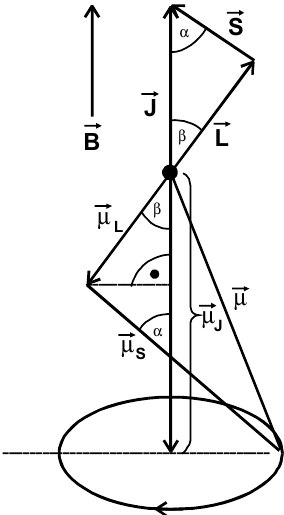
\includegraphics[width=0.45\textwidth]{ressources/Theorie1.png}
	\caption{}
	\label{fig:Theorie1}
\end{subfigure}%
\begin{subfigure}{.5\textwidth}
	\centering
	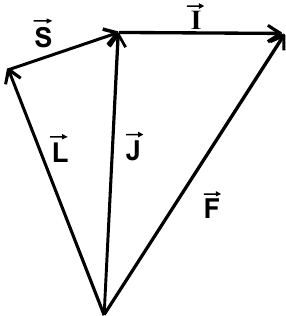
\includegraphics[width=0.45\textwidth]{ressources/Theorie2.png}
	\caption{}
	\label{fig:Theorie2}
\end{subfigure}
\caption{Geometrische Anordnung der zuvor beschriebenen Drehimpulse und den dazugehörigen magnetischen Momenten. \cite{skript}}
\label{fig:geoAnordnung}
\end{figure}

Aufgrund einer Präzessionsbewegung um die Gesamtdrehimpulsrichtung $\vec{J}$ mitteln sich alle senkrecht dazu stehenden Komponenten des magnetischen Moments $\vec{\mu}_J$  zeitlich heraus (siehe Abbildung \ref{fig:Theorie1}). Aus den Beträgen der magnetischen Momente

\begin{align}
	|\vec{\mu}_S|&=g_S\mu_B\sqrt{S(S+1)} \\
	|\vec{\mu}_L|&=\mu_B\sqrt{L(L+1)}\\
	|\vec{\mu}_J|&=g_J\mu_B\sqrt{J(J+1)}
	\label{eq:betragmu1}
\end{align}

folgt nach Abbildung \ref{fig:Theorie2} der geometrische Zusammenhang

\begin{align}
	|\vec{\mu}_J| &= |\vec{\mu}_L| \cos{(\beta)}+ |\vec{\mu}_S| \cos{(\alpha)}\;.
	\label{eq:betragJ}
\end{align}

Mit dem magnetische Moment des Kerns
\begin{align}
	|\vec{\mu}_I|&=g_I\mu_k\sqrt{I(I+1)}
\end{align}
und Gleichung \ref{eq:betragJ} berechnet sich das magnetische Moments des Atoms unter Berücksichtigung von Abbildung \ref{fig:Theorie2}
zu 
\begin{align}
	|\vec{\mu}_F|&=|\vec{\mu}_J|\cos{(\vec{J},\vec{F})} + |\vec{\mu}_I|\cos{(\vec{I},\vec{F})}\;.
	\label{eq:betragF}
\end{align}

Der zweite Summand wird aufgrund des Massenunterschieds zwischen Nukleon und Elektron ($\mu_K<<\mu_B$) vernächlässigt. Mit dem Kosinussatz ergibt sich schlussendlich für den Land\'{e}-Faktor des Kerns
\begin{align}
	g_F \approx g_J \frac{F(F+1)+J(J+1)-I(I+1)}{2F(F+1)}\;.
	\label{eq:11}
\end{align}


\subsection{Zeeman-Effekt}
In einem äußeren Magnetfeld wechselwirkt das magnetische Moment mit dem Feld. Die dabei entstehende potentielle Energie wird als Wechselwirkungsenergie bezeichnet. Da nur die zum Feld parallel Komponenten von $\vec{\mu}$ relevant sind, kann aufgrund der Richtungsquantelung das magnetische Moment durch die Orientierungsquantenzahl $M_J$ ersetzt werden, sodass folgt 
\begin{align}
	U_\textrm{mag}&=-\vec{\mu}_J \vec{B}=M_Jg_J\mu_BB\;.
	\label{eq:7}
\end{align}

Durch den Elektronenspin und der Wechselwirkung mit dem Drehimpuls des selben, spalten sich die Energieniveaus auf. Liegt zudem ein nicht verwindender Kernspin vor, erfolgt eine weitere Aufspaltung. Schlussendlich erfolgt eine dritte, die durch das Anlegen eines äußeres Magnetfelds in Erscheinung tritt, den zuvor beschriebenen Zeeman-Effekt. Zusammenfassend entstehende drei Bereiche: die Feinstruktur, die Hyperfeinstruktur und die Zeeman-Aufspaltung (vlg. Abbildung \ref{fig:Aufspaltung}).

\begin{figure}
	\centering
	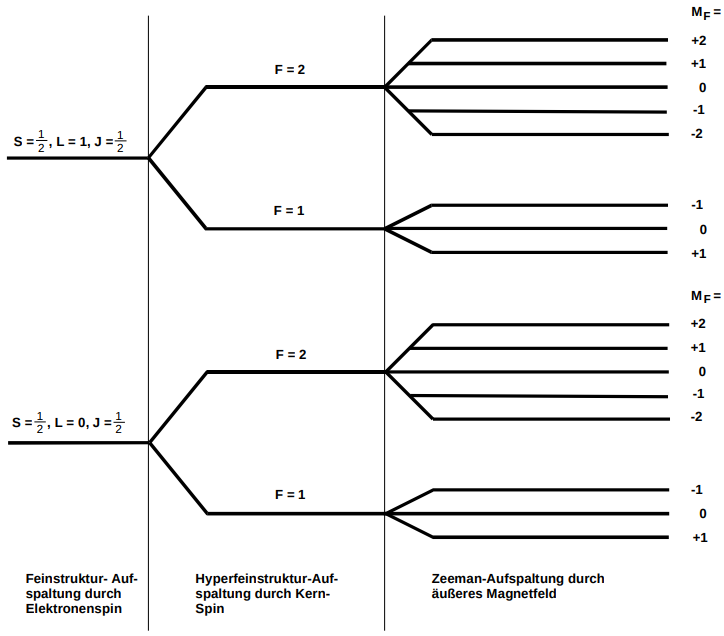
\includegraphics[width=0.55\textwidth]{ressources/Aufspaltung.png}
	\caption{Aufspaltung der Energieniveaus unterteilt in die Bereiche der Feinstruktur, der Hyperfeinstruktur und der Zeeman-Aufspaltung. \cite{skript}}
	\label{fig:Aufspaltung}
\end{figure}

Die Energiedifferenz zwischen den Niveaus beträgt
\begin{align}
	U_\textrm{HF}=g_F\mu_BB,
	\label{eq:8}
\end{align}
wobei durch hohe Magnetfelder die Spin-Bahn-Wechselwirkung einen immer größeren Einfluss hat. Die Näherung der Energiedifferenz in zweiter Ordnung wird als Breit-Rabi-Formel bezeichet
\begin{align}
	U_\textrm{HF}=g_F\mu_BB+g_F^2\mu_B^2B^2\frac{(1-2M_F)}{\Delta E_\textrm{Hy}},
	\label{eq:16}
\end{align}
wobei $\Delta E_\textrm{Hy}$ die Energiedifferenz der Hyperfeinstruktur zwischen den Niveaus mit den Quantenzahlen $F$ und $F+1$ beschreibt.

\subsection{Optisches Pumpen}
\label{sec:optischesPumpen}
Befinden sich zwei Zustände im thermischen Gleichgewicht, ist der energetisch niedrigere Zustand stärker besetzt als der energetisch höhere. Das Prinzip des optischen Pumpen sieht vor diesen Besetzungszustand zu invertieren. Anhand der von Abbildung \ref{fig:optischesPumpen} soll dieses Prinzip beschrieben werden.

\begin{figure}
	\centering
	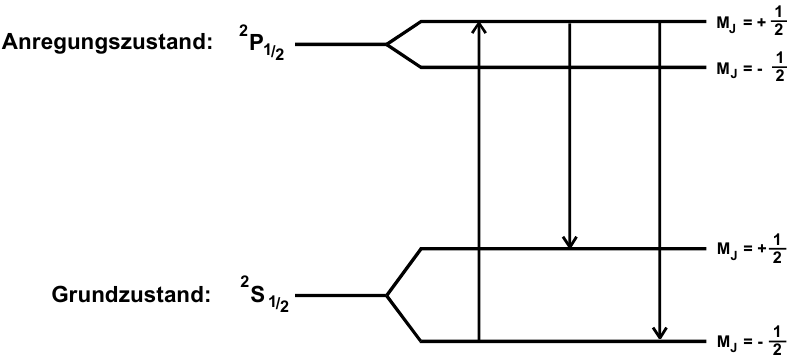
\includegraphics[width=0.55\textwidth]{ressources/optischesPumpen.png}
	\caption{Aufspaltung der Energieniveaus eines Alkali-Atoms mit eingezeichneten erlaubten Übergängen, die durch Anregung bzw. spontane Emission verursacht werden. \cite{skript}}
	\label{fig:optischesPumpen}
\end{figure}

Für das erreichen einer Inversion wird rechtszirkular-polarisiertes Licht eingestrahlt. Aufgrund der Auswahlregel $\Delta M_J=+1$ gehen die Zustände vom Grundzustand $\ce{^{2}_{}S_{1/2}}$ $(M_J=-\frac{1}{2})$ in den angeregten Zustand $\ce{^{2}_{}P_{1/2}}$ $(M_J=+\frac{1}{2})$ über. Die Zustände in Grundzustand $\ce{^{2}_{}S_{1/2}}$ $(M_J=+\frac{1}{2})$ werden nicht angeregt, da kein Zustand existiert, der die Auswahlregel erfüllt. Im angeregten Zustand  $\ce{^{2}_{}P_{1/2}}$ $(M_J=+\frac{1}{2})$ befindliche Zustände gehen durch spontane Emission, bei der ein Photon emittiert wird, wieder in den Grundzustand über. Dabei ist es gleich wahrscheinlich, dass der Übergang in den Zustand $\ce{^{2}_{}S_{1/2}}$ 
$(M_J=-\frac{1}{2})$ und $\ce{^{2}_{}S_{1/2}}$ $(M_J=+\frac{1}{2})$ stattfindet. Somit wird der Grundzustand $\ce{^{2}_{}S_{1/2}}$ $(M_J=-\frac{1}{2})$ leer "gepumpt" und es entsteht zu $\ce{^{2}_{}S_{1/2}}$ $(M_J=+\frac{1}{2})$ eine Besetzungszahlinversion.

\subsection{Hochfrequenz-Spektroskopie}
Das im Kapitel \ref{sec:optischesPumpen} angesprochene Verfahren kann unter anderem dazu verwendet werden, die Abstände zwischen zwei Energieniveaus zu vermessen.
Grundsätzlich gibt es zwei Möglichkeiten wie Elektronen, nachdem sich eine Besetzungsinversion eingestellt hat, vom "vollgepumpten" Zustand in den Grundzustand übergehen können. Die erste Möglichkeit besteht in der spontanen Emission. Dabei wird ohne eine Einwirkung von außen ein Photon emittiert. Die Energie des Photons gleicht dabei der Energiedifferenz der beiden betrachteten Zuständen. Bei der zweiten Möglichkeit, der induzierten Emission, wird ein durch ein Hochfrequenzfeld erzeugtes Photon eingestreut. Daraufhin wird ein in Polarität, Frequenz und Energie gleiches Photon emittiert und der Zustand geht in der Grundzustand über. Die dafür benötigte Energie des eingestrahlten Photons entspricht
\begin{align}
	h\nu&=g_J\mu_BB_m\Delta M_J\;.
	\label{eq:hnu}
\end{align}
Welcher der beiden Möglichkeiten dominiert ist Frequenzabhängig, in dem vorliegenden Fall kann die spontane Emission vernachlässigt werden.
Um die Breite der Energielücke zu bestimmen wird die Transparenz ausgenutzt, diese entsteht, wenn einfallende Photonen nicht mehr absobiert werden. In dem vorliegenden Fall tritt dieses auf, wenn der Grundzustand "leer gepumpt" wurde und das hier verwendete  $\ce{^{87}_{}Rb}$ und $\ce{^{85}_{}Rb}$ somit transparent wird. In Abbildung \ref{fig:TransparenzZeit} ist die entstehende Transparenz gegen die Zeit aufgetragen.


\begin{figure}
	\centering
	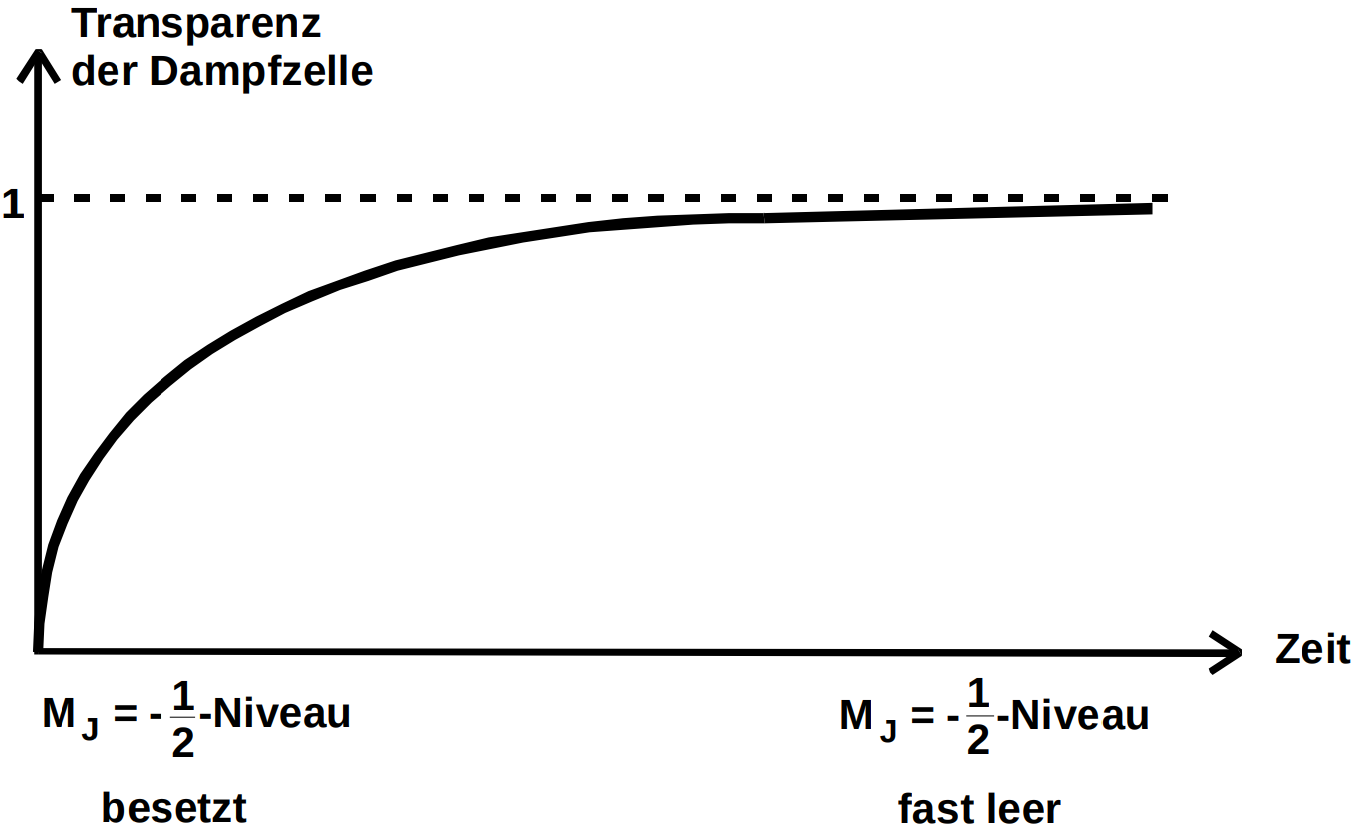
\includegraphics[width=0.475\textwidth]{ressources/TransparenzZeit.png}
	\caption{Verlauf der Transparenz in einer Alkali-Dampfzelle gegen die Zeit, in der $D_1$-Licht eingestrahlt wird. \cite{skript}}
	\label{fig:TransparenzZeit}
\end{figure}


Zur Bestimmung der Breite der Bandlücke wird nun die Resonanzstelle gesucht, die sich in der Transparenz wiederspiegelt. In Abbildung \ref{fig:Resonanz} ist dieses Verhalten bei variierenden Magnetfeld dargestellt.

\begin{figure}
	\centering
	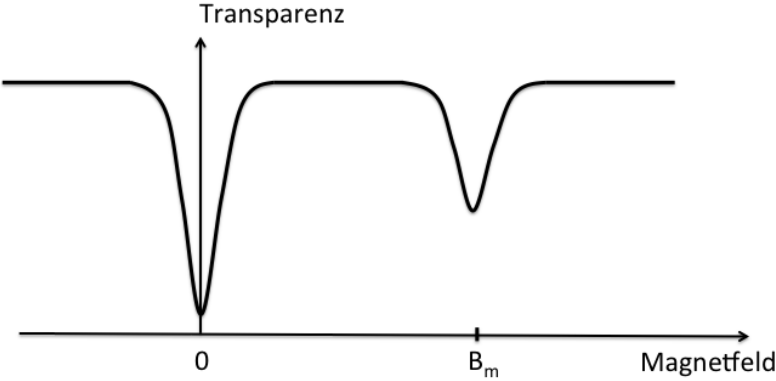
\includegraphics[width=0.475\textwidth]{ressources/Resonanz.png}
	\caption{Verlauf der Transparenz in einer Alkali-Dampfzelle gegen das Magnetfeld, bei angelegtem Hochfrequenzfeld. \cite{skript}}
	\label{fig:Resonanz}
\end{figure}

Bei verschwindendem Magnetfeld findet keine Zeeman-Aufspaltung statt, wodurch bei $B=0$ die Transparenz auf Null absingt. Mit der zweiten Resonanzstelle und Gleichung \ref{eq:hnu} kann die somit die Breite der Bandlücke bestimmt werden.







% 2x2 Plot
% \begin{figure*}
%     \centering
%     \begin{subfigure}[b]{0.475\textwidth}
%         \centering
%         \includegraphics[width=\textwidth]{Abbildungen/Schaltung1.pdf}
%         \caption[]%
%         {{\small Schaltung 1.}}
%         \label{fig:Schaltung1}
%     \end{subfigure}
%     \hfill
%     \begin{subfigure}[b]{0.475\textwidth}
%         \centering
%         \includegraphics[width=\textwidth]{Abbildungen/Schaltung2.pdf}
%         \caption[]%
%         {{\small Schaltung 2.}}
%         \label{fig:Schaltung2}
%     \end{subfigure}
%     \vskip\baselineskip
%     \begin{subfigure}[b]{0.475\textwidth}
%         \centering
%         \includegraphics[width=\textwidth]{Abbildungen/Schaltung4.pdf}    % Zahlen vertauscht ... -.-
%         \caption[]%
%         {{\small Schaltung 3.}}
%         \label{fig:Schaltung3}
%     \end{subfigure}
%     \quad
%     \begin{subfigure}[b]{0.475\textwidth}
%         \centering
%         \includegraphics[width=\textwidth]{Abbildungen/Schaltung3.pdf}
%         \caption[]%
%         {{\small Schaltung 4.}}
%         \label{fig:Schaltung4}
%     \end{subfigure}
%     \caption[]
%     {Ersatzschaltbilder der verschiedenen Teilaufgaben.}
%     \label{fig:Schaltungen}
% \end{figure*}
